\documentclass[palatino]{apuntes}

\usepackage[usenames,dvipsnames]{xcolor}
\usepackage{longtable}
\usepackage{fancysprefs}
\usepackage{minted}
\usepackage{showexpl}
\usepackage{etoolbox}
\usepackage{booktabs}

\definecolor{lightgrey}{gray}{0.95}

\lstset{basicstyle=\footnotesize\ttfamily}

\lstset{language=[LaTeX]TeX,
	texcsstyle=*\bf\color{blue},
	numbers=none,
	breaklines=true,
	keywordstyle=\color{darkgreen},
	commentstyle=\color{red},
	frame=none,
	tabsize=2,
	backgroundcolor=\color{lightgrey}
}

\makeatletter
\newlength{\parindent@save}
\AtBeginDocument{\setlength{\parindent@save}{\parindent}}
\patchcmd{\SX@put@code@result}% <cmd>
  {\SX@resultInput}% <search>
  {\setlength{\parindent}{\parindent@save}\SX@resultInput}% <replace>
  {}{}% <success><failure>
\makeatother

\author{Guillermo Julián Moreno}
\date{\today}
\title{\LaTeX\ para infomates}

\setcounter{tocdepth}{3}

\begin{document}

\begin{abstract}
Este documento pretende ser un manual de uso de \LaTeX\ y de los paquetes personalizados que tenemos para escribir los \href{http://github.com/VicdeJuan/Apuntes}{apuntes de matemáticas e informática}.  La idea es que sirva para aprender \LaTeX\ básico (\fref{chap:Introduccion}), que introduzca aspectos de \LaTeX\ avanzado (\fref{chap:LaTeXAvanzado}) y que documente los paquetes y comandos personalizados que hemos ido desarrollando a lo largo del tiempo (\fref{chap:PaqueteExtendido}).
\end{abstract}

\pagestyle{plain}
\maketitle

\newpage

\tableofcontents


\chapter{Una introducción a \LaTeX}
\label{chap:Introduccion}

Vayamos primero con las preguntas básicas: ¿qué es \LaTeX? Es un sistema de generación de documentos\footnote{En inglés, \textit{document typesetting system}, que queda mejor.}. En otras palabras, nosotros escribimos cosas y \LaTeX\ nos genera un documento como este mismo manual.

La siguiente pregunta es: ¿por qué usar \LaTeX\ y no Word o LibreOffice? Esta pregunta ya no tiene una respuesta tan clara, aunque podemos comentar algunas ventajas. Por ejemplo, es mucho más fácil obtener documentos maquetados a la perfección: \LaTeX\ nos permite despreocuparnos del formato mientras escribirmos porque él se encarga de todo: gestión de los párrafos, tamaño de fuente\footnote{A modo de curiosidad sobre las fuentes, una de las razones por las que \LaTeX\ saca documentos tan ``profesionales'' es lo que se llama el \textit{font kerning} o espaciado entre letras. Por si alguien quiere saber más, \href{http://nitens.org/taraborelli/latex}{este artículo en inglés es bastante interesante}.} para cada posible situación, colocación de los imágenes, saltos de página, numeración\ldots Básicamente, todo lo que se pueda automatizar se automatiza, mientras que nosotros nos preocupamos de lo importante: escribir. Además, no hace falta saber cómo maquetar bien los documentos para que nos queden bien, y además la mejor forma de hacer algo es siempre la más fácil.

Por supuesto, esto viene con un coste, y es que \LaTeX\ no es fácil. Sólo hay que ver que estás leyendo un manual para aprender: ¿cuándo has leído un manual para usar Word?

La razón por la que no es fácil es que con \LaTeX\ no escribimos letras, pulsamos botones y ya. En \LaTeX\ lo que se hace es escribir comandos y compilar el documento para generar algo legible, así que podemos decir que se parece bastante a programar. Por ejemplo, cuando queremos poner algo en negrita, no nos vamos al botón correspondiente en el programa: lo que hacemos es escribir el comando correspondiente (\verb|\textbf{negrita}|) para que cuando el compilador pase por ahí, sepa que tiene que poner esas palabras en negrita.

Esto tiene una cosa mala, y es que escribir un documento \textit{.tex} puede llegar a ser un poco infernal, porque ves los comandos y no lo que producen. Otro problema es que, al escribir comandos, puedes equivocarte y que el documento no compile. No sería un problema demasiado importante si no fuese porque la mitad de las veces los errores que muestra un compilador son complementamente inútiles. Más tarde veremos cómo enfrentarnos a esos errores de compilación, pero primero empezaremos por lo más interesante: nuestro primer documento \LaTeX{}.

\section{Hola Mundo: Primer documento con \LaTeX}

Decíamos antes que \LaTeX\ necesita un compilador, así que antes de nada vamos a necesitar instalarlo. También instalaremos un editor especializado. Aunque no es necesario (los documentos \textit{.tex} son texto plano que se pueden editar hasta con el bloc de notas), sí que nos vendrá muy bien para empezar, ya que nos facilitan mucho la vida con una interfaz amable y botones que hacen las cosas por nosotros.

\subsection{Instalando un entorno \LaTeX}

Lo que necesitaremos bajarnos en nuestro ordenador será una \textit{distribución \LaTeX}, que es una colección de programas y archivos de configuración que nos permitirán generar nuestros documentos. Según el sistema que usemos, tendremos que bajarnos una cosa u otra:

\begin{itemize}
\item \textbf{Windows}. Antes de decir cómo descargarse \LaTeX, haré una recomendación, y es que Windows no es el sistema más apropiado para esto, sobre todo si queremos editar los apuntes de infomates. Es mejor irse a un sistema POSIX (Linux o Mac OS X) que tenga una consola decente y con \textit{bash} para poder ejecutar los \textit{scripts} que tenemos en el repositorio. Además, estudiando informática, se acaba usando Linux sí o sí, así que cuanto antes se empiece a usarlo mejor. Si a pesar de todo queremos seguir con Windows, lo que hay que bajarse es \href{http://miktex.org/download}{la distribución MikTeX} e instalarla (es un instalador normal y corriente).

\item \textbf{Mac OS X}. Hay varias formas de instalarse \LaTeX\ en OS X, aunque yo recomiendo usar Macports\footnote{Macports es un gestor de paquetes al estilo \textit{apt-get} para OS X. \href{https://www.macports.org/install.php}{Estas son las instrucciones para instalarlo}.} e instalar los paquetes necesarios con \texttt{sudo port install texlive-basic texlive-bin-extra texlive-fonts-extra texlive-lang-spanish texlive-latex texlive-latex-extra texlive-math-extra}.

\item \textbf{Linux basado en Debian (Ubuntu y similares)}. El paquete básico para usar \LaTeX\ es \textit{texlive}, así que con \texttt{sudo apt-get install texlive} debería bastar. Es recomendable bajarse además \textit{texlive-latex-base, texlive-latex-extra, texlive-latex-recommended} para paquetes adicionales que no están en la distribución base.

\item \textbf{Linux no basado en Debian}. Como de estos hay muchos y los que se lo instalan suelen ser un poco más apañados que la media, daré por supuesto que sabrán encontrar los paquetes que necesitan instalar sabiendo los que necesita Ubuntu.
\end{itemize}

\index{TeXStudio}
Una vez que tenemos \LaTeX\ instalado, nos bajaremos el editor. Personalmente, recomiendo \href{http://www.texstudio.org/}{TeXStudio}, que funciona bastante bien, es fácil de usar y además es bastante potente.

\subsection{Un primer documento}
\label{sec:EstructuraDocumento}

Una vez que tenemos todo instalado, podemos hacer nuestro primero documento. El archivo está \href{https://github.com/VicdeJuan/Apuntes/blob/master/Cosas%20guays%20LaTeX/Manual/DocumentoMuestra.tex}{disponible para que que se pueda descargar y bajar} sin tener que copiar y pegar de un PDF.

\inputminted[linenos,tabsize=2,fontsize=\footnotesize, breaklines]{latex}{DocumentoMuestra.tex}

\begin{figure}[hbtp]
\centering
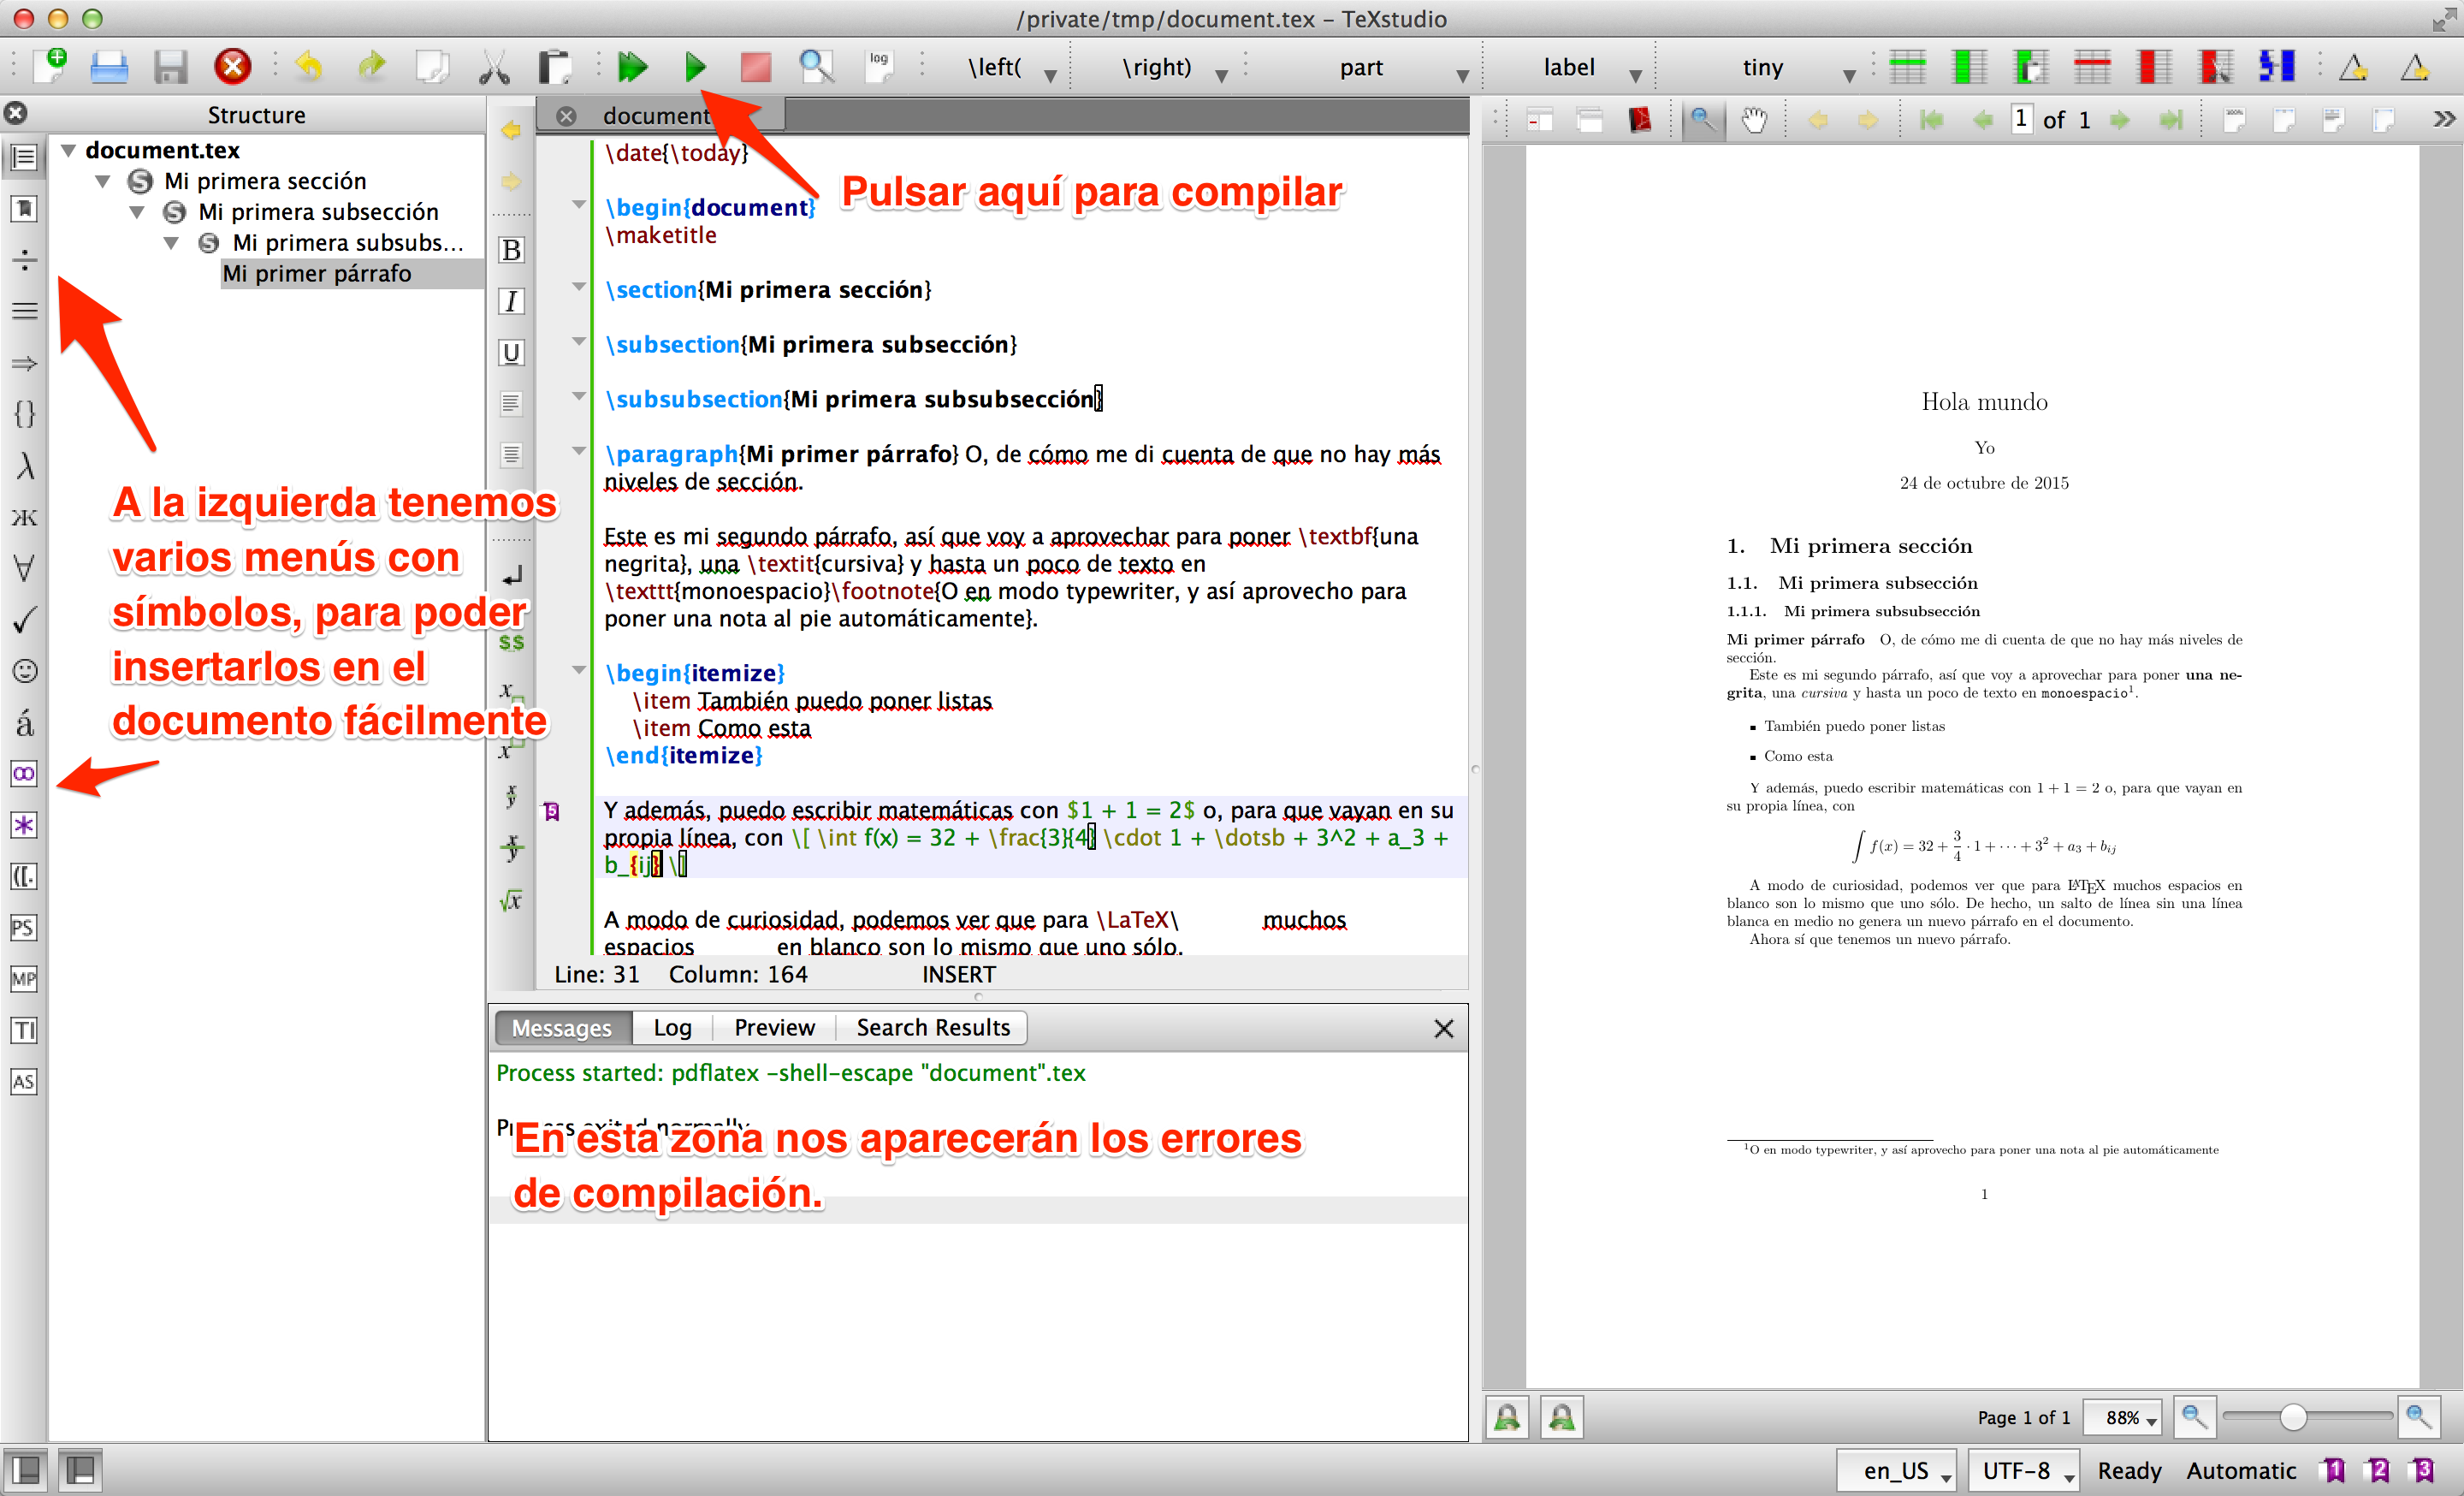
\includegraphics[width=\textwidth]{TeXStudio.png}
\caption{Una captura de pantalla de TeXStudio con el documento de muestra, junto con algunas indicaciones sobre la interfaz.}
\label{fig:TeXStudio}
\end{figure}

Es recomendable toquetear el documento y ver qué pasa si quitamos comandos, o si cambiamos letras. La \fref{fig:TeXStudio} muestra cómo queda este documento si lo vemos en TeXStudio.

En este documento podéis ver varios comandos (los que empiezan por ``\verb|\|''), de los cuales muchos no merecen demasiada explicación. Otros los veremos más tarde, como los relacionados con ecuaciones matemáticas.

Lo que sí vamos a comentar son los comandos \verb|\documentclass|, \verb|\usepackage|  y los \verb|\begin{document}| y \verb|\end{document}|. El primero debería estar siempre en la primera línea de cualquier documento \LaTeX, y le dice al compilador qué tipo de documento estamos escribiendo. En este caso es \textit{article}, aunque podría ser cualquier otro como \textit{book} o \textit{report}. El tipo de documento definirá qué márgenes usamos, el tipo de letra, los tipos de secciones que se pueden usar o los paquetes que se incluyen por defecto.

\index{usepackage}
\index{documentclass}
Eso nos lleva al siguiente comando, \verb|\usepackage|. Como su nombre indica, carga un paquete en el documento y siempre van en el preámbulo (ahora veremos qué es eso). Un paquete de \LaTeX\ puede o bien proporcionarnos comandos (por ejemplo, \textit{amsmath} nos proporciona los comandos \verb|\int| o \verb|\dotsb|) o bien cambiar el comportamiento de \LaTeX, como \textit{babel}, que con la opción \textit{spanish} traducirá las cadenas que el compilador inserte en el documento (por ejemplo, cuando ponga la fecha automáticamente o cuando ponga ``Figura N'' en las etiquetas de imágenes) en español.

Por último, nos quedan los comandos \verb|\begin{document}| y \verb|\end{document}|. Son un ejemplo de lo que se llaman ``entornos'' en \LaTeX. Como uno podría imaginar, marcan el inicio y el final del documento en sí. Lo que esté dentro de estos dos comandos es lo que se ve en el documento final. Lo que está fuera (antes del \verb|\begin{document}|, porque después de \verb|\end{document}| no debería haber nada) es lo que se llama el preámbulo, que podríamos decir que es la sección de ``configuración'' del documento.

\section{Formato y maquetación}

Ahora que ya sabemos a grandes rasgos cómo funciona un documento \LaTeX, vamos a ir viendo explicaciones más en detalle de cada aspecto, empezando por lo básico: cómo dar formato y maquetar nuestro documento.

\subsection{Dando estructura: secciones, subsecciones, párrafos y más}

\index{Tabla!de contenidos}
\index{Sección}
Normalmente, los documentos se organizan en secciones, subsecciones y similares. \LaTeX{} nos lo pone muy fácil para hacerlo. Sólo necesitaremos poner el comando correspondiente y se encargará de ponerle el número que le corresponda y de añadirlo a la tabla de contenidos si la hemos activado. Para que la tabla de contenidos nos aparezca en el documento, sólo tenemos que escribir \verb|\tableofcontents| donde queramos que se muestre.

\index{chapter}
Las posibles variantes de sección son las siguientes. Como aparece en el comentario, el comando \verb|\chapter| sólo se puede usar en algunos tipos de documento, como \textit{report} o \textit{book} (no \textit{article}).

\begin{minted}{latex}
\chapter{Un capítulo} % Sólo en algunos tipos de documento
\section{Una sección}
\subsection{Una subsección}
\subsubsection{Una subsubsección}

\paragraph{Un párrafo}

\subparagraph{Un subpárrafo}
\end{minted}

\index{Párrafo}
Además, como indicábamos en el documento de muestra, \LaTeX\ es algo especialito con los espacios en blanco y los párrafos. Varios espacios en blanco es lo mismo que uno sólo, y los saltos de línea se ignoran salvo que haya una línea en blanco, que es lo que indica a \LaTeX\ que hay un nuevo párrafo.

Si se quiere forzar un salto de línea (no recomendado, \LaTeX\ sabe mejor que cualquiera de nosotros cómo y donde romper las líneas; y si quieres cambiar de párrafo deberías poner una línea en blanco) podemos usar \verb|\\|, \verb|\newline| o \verb|\pbreak|.

\begin{LTXexample}[pos=r]
Esta linea
y esta otra
son del mismo parrafo.

Ahora si cambiamos de parrafo, y tambien podemos ver que
los       espacios dan igual, con uno basta.

El cambio de linea forzado queda un poco mas raro y \\
no cambia bien de
parrafo. Es mejor no usarlo.
\end{LTXexample}

\subsection{Dando formato: negritas, cursivas y demás tipo de letra}

\index{Cursiva}
\index{Negrita}
Una revisión rápida por los posibles tipos de letra que podemos tener:

\begin{LTXexample}[pos=r]
\textbf{negrita}, \textit{cursiva}, \texttt{monoespacio}

\Huge{muy enorme}, \huge{enorme},
\LARGE{muy muy grande},
\Large{muy grande}, \large{grande},
\normalsize{normal}, \small{reducido},
\tiny{muy reducido}.
\end{LTXexample}

\index{Verbatim}
También podemos querer escribir código y no preocuparnos porque \LaTeX\ lo trate de interpretar. Para eso podemos usar los entornos \textit{verbatim}:

\begin{LTXexample}[pos=r]
En el texto, podemos usar
\verb|\micomando| (atentos
a las barras verticales para
delimitar el argumento)
para que \LaTeX{}
no trate de interpretar lo
que ponemos como un comando.

Si queremos algo mas extenso
podemos usar el entorno
\textit{verbatim}:

\begin{verbatim}
\textit{LaTeX no interpreta esto}
\end{verbatim}
\end{LTXexample}

\subsection{Otros entornos}

Lo último que vamos a ver de formato y maquetación en \LaTeX\ será cómo meter listas, imágenes y tablas en nuestros documentos.

\subsubsection{Listas}

\index{Lista}
Las listas son sencillas, y lo mejor es verlo con ejemplos. Por supuesto, las listas se pueden anidar.

\begin{LTXexample}[pos=r]
\begin{itemize}
\item Uno
\item Dos
\end{itemize}

\begin{enumerate}
\item Numerado
\item Por defecto
\begin{enumerate}
\item Incluso con anidaciones
\item Podemos poner todos los niveles
\begin{enumerate}
\item Que queramos
\end{enumerate}
\item \LaTeX{} hace todo
\end{enumerate}
\item De forma automatica.
\end{enumerate}

\begin{description}
\item[Etiqueta] Elemento
\end{description}
\end{LTXexample}

\subsubsection{Imágenes}
\label{sec:Imagenes}

\index{Imagen}
\index{includegraphics}
Para poner imágenes, sólo es necesario un comando, \verb|\includegraphics|. La cuestión es que eso nos inserta la imagen directamente, y no nos permite poner una etiqueta ni referenciarlo más tarde. Lo que haremos será encerrar ese comando en un entorno \textit{figure}:

\begin{LTXexample}[pos=r]
\begin{figure}[hbtp]
\centering
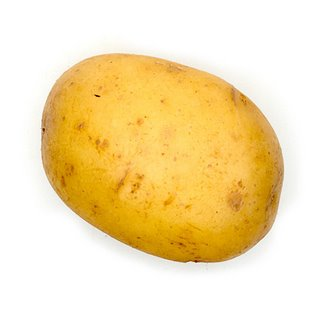
\includegraphics[width=0.4\textwidth]{Patata.jpg}
\caption{Etiqueta para la figura}
\label{fig:FiguraEjemplo}
\end{figure}
\end{LTXexample}

El entorno \textit{figure} es lo que se llama un entorno flotante. La ventaja es que nos da opciones adicionales y además le dice a \LaTeX\ que coloque la imagen donde sea más conveniente, evitando dejar muchos espacios en blanco o rompiendo el flujo del texto. Esta es una de las cosas que más cambian con respecto a Word, y de lo que más cuesta convencer: es mejor dejar que \LaTeX\ ponga la imagen donde quiera: normalmente será una posición mejor que la que podamos poner nosotros, y además nos evitaremos dolores de cabeza cuando cambiemos el texto y se nos descuadren todas las imágenes (como en Word).

Lo que sí podemos decirle a \LaTeX\ es donde preferimos que ponga la imagen (luego nos hará caso o no) con las opciones \texttt{[hbtp]}. Cada letra denota una preferencia, y van ordenadas según su prioridad: primero intenta poner la imagen donde la has escrito; si no puede, en la parte inferior de la página; si no, en la parte superior; y si ahí tampoco puede la dejará en una página dedicada a imágenes. Las letras se pueden quitar y cambiar de orden según querramos que aparezca la imagen.

El comando \verb|\includegraphics[width=X\textwidth]{ruta/a/la/imagen}| es el que inserta la imagen en sí. Normalmente solemos limitar el ancho de la imagen con la opción \verb|[width=X\textwidth]|, donde $X$ es el porcentaje (entre 0 y 1) del ancho del texto que queremos que ocupe. Por ejemplo, \verb|0.5\textwidth| hará que la imagen ocupe la mitad del texto de ancho.

\index{caption}
\index{label}
El comando \verb|\caption| nos permite ponerle una etiqueta o ``caption'' a la imagen, para explicar qué es. Es conveniente usarlo, porque siempre se mantiene pegado a la imagen y además nos permite ver qué índice tiene la figura. Por último, el comando \verb|\label| le asigna un identificador a la figura para que podamos referenciarla más tarde (veremos cómo hacer eso en la \fref{sec:Etiquetas}).

\subsubsection{Tablas}
\label{sec:Tablas}

\index{Tabla}
\index{tabular}
\LaTeX\ también nos permite incluir tablas en los documentos, aunque no es especialmente cómodo. Necesitaremos usar el entorno \textit{tabular}, al que le especificamos las columnas que queremos usar. Después, ponemos los contenidos de la tabla, separando cada celda con el carácter \verb|&| y cada fila con el salto de línea \verb|\\|. Veamos un ejemplo:

\begin{LTXexample}[pos=r]
\begin{tabular}{rl|r|c||}
0 & 1 & 2 & 3 \\ \hline
texto & texto & texto & texto
\end{tabular}
\end{LTXexample}

\index{hline}
El primer argumento de \textit{tabular} es el especificador de columnas. Normalmente son los caracteres \textit{r,l,c}, que indican alineación de la celda a la derecha, a la izquierda o al centro respectivamente; y separados (o no) por caracteres \texttt{|}, que le dicen a \LaTeX\ que ponga una barra vetical entre esas dos columnas. Para poner barras horizontales, ponemos el comando \texttt{hline} al final de la línea.

Al igual que con las imágenes, la mayor parte de las veces nos interesará poner la tabla en un entorno flotante, \textit{table}, para que \LaTeX\ la coloque donde mejor venga y podamos poner un \textit{caption} y la referencia con \textit{label}.

\begin{LTXexample}[pos=r]
\begin{table}[hbtp]
\centering
\begin{tabular}{rl|r|c||}
0 & 1 & 2 & 3 \\ \hline
texto & texto & texto & texto
\end{tabular}
\caption{Etiqueta para la tabla}
\label{tbl:TablaEjemplo}
\end{table}
\end{LTXexample}

\section{Matemáticas en \LaTeX}

Habiendo llegado hasta aquí, ya deberíamos de saber generar documentos básicos en \LaTeX. Ahora bien, nos falta una de las características más potentes de este sistema, y que siendo infomates debería interesarnos mucho: escribir matemáticas.

\LaTeX\ tiene lo que se llama un ``modo matemáticas'', donde dejará de interpretar texto e interpretará los símbolos que pongamos como lo que son: ecuaciones y fórmulas matemáticas. Los principales son dos, aunque hay bastantes más. Por un lado, los dólares (\$) nos permiten poner ecuaciones en línea, en el párrafo. Por otro, con \verb|\[.. \]| \LaTeX\ nos pondrá la ecuación en una línea separada. Veamos un ejemplo.

\begin{LTXexample}[pos=r]
Podemos poner ecuaciones $1 = 2$
en linea, o tambien separadas con
\[ 1 = 2 + 4 \]

No hace falta poner el salto de
linea, se hace solo. Si escribimos
asi \[ 1 = \int 3 \] el salto es
automatico. De hecho, LaTeX no
cambia de parrafo.
\end{LTXexample}

A modo de aviso, en muchos sitios todavía se sigue usando dos dólares (\$\$) en lugar de los corchetes. No deberían usarse (es sintaxis antigua), y además puede dar algunos errores y generar text que no queda del todo bien.

Para usar matemáticas en un documento \LaTeX, es recomendable incluir el paquete \textit{amsmath}, que añade bastantes comandos y mejora el funcionamiento de las ecuaciones.

\subsection{Subíndices y superíndices, fracciones y raíces}

Para poner subíndices y superíndices, usaremos los caracteres \verb|_| y \verb|^| respectivamente. Por ejemplo:

\begin{LTXexample}[pos=r]
\[ a_b + 3^2 \]
\[ a_bj + a_{bj} + 3^{2i} + 3^2i\]
\end{LTXexample}

Hay que tener cuidado cuando querramos poner subíndices o superíndices con más de dos caracteres: en ese caso, hay que rodearlos con llaves porque si no \LaTeX\ sólo pone el primer carácter.

\index{Fracción}
\index{Raíz}
Las fracciones se ponen con el comando \verb|\frac{numerador}{denominador}|, o \verb|\dfrac| si estamos en modo \textit{inline} (con \$...\$) y queremos que la fracción no aparezca en tamaño pequeño.

Para poner raíces usaremos el comando \verb|\sqrt|, que como argumento opcional acepta el orden de la raíz:

\begin{LTXexample}[pos=r]
Las fracciones en el texto $\frac{1}{2}$
aparecen reducidas, cosa que
podemos corregir con $\dfrac{3}{4}$.

\[ \frac{3 + 2}{5} = 1 = \sqrt{1} = \sqrt[3]{1}\]
\end{LTXexample}

\subsection{Matrices}

Las matrices en \LaTeX\ tienen una sintaxis parecida a las tablas (\fref{sec:Tablas}): separamos las celdas por \verb|&| y las filas por \verb|\\|. La diferencia está en que usamos el entorno \textit{matrix} (o sus variantes \textit{pmatrix} o \textit{vmatrix}):

\begin{LTXexample}[pos=r]
\[
\begin{matrix}
1 & 2 \\
3 & 4
\end{matrix} =
\begin{pmatrix}
1 & 2 \\ 3 & 4
\end{pmatrix} =
\begin{vmatrix}
1 & 2 \\ 3 & 4
\end{vmatrix}
\]
\end{LTXexample}

\subsection{Delimitadores}

\index{left}
\index{right}
En ocasiones querremos introducir delimitadores, como paréntesis o llaves, en las ecuaciones. Normalmente funcionan bien, salvo cuando queremos meter cosas más grandes dentro (por ejemplo, un símbolo de sumatorio) que se quedan limitadores demasiado pequeños. Para evitar eso usaremos los comandos \verb|\left| y \verb|\right| seguidos de un carácter que \LaTeX\ cambiará de tamaño para que se ajuste bien. Si por lo que sea queremos que uno de los lados no tenga ningún delimitador, podemos usar un punto. Veámoslo claro con un ejemplo:

\begin{LTXexample}[pos=r]
\[ (1 + 2) = 3\]
\[ (\frac{3}{4} + 4) = \left(\frac{3}{4} + 1 \right)\]

% Podemos tener delimitadores distintos
% o incluso quitar uno de ellos con '.'
\[ \left(\sum \right] = \left(\int \right. \]
\end{LTXexample}

Siempre hay que acordarse de cerrar bien los delimitadores: si nos dejamos un \verb|\left| sin su correspondiente \verb|\right| (o viceversa) \LaTeX\ nos dará un error de compilación un poco raro.

\subsection{Símbolos, operadores y texto}
\label{sec:SimbolosOperadoresTexto}

Es obvio que, salvo unos pocos casos, necesitaremos símbolos complejos para nuestras ecuaciones. Prácticamente todos están definidos como comandos, incluyendo las letras griegas. Algunos, como los comandos de límite, integral o sumatorio, colocan los superíndices y subíndices correctamente cuando los ponemos. Veamos ejemplos de esos símbolos (\href{https://en.wikibooks.org/wiki/LaTeX/Mathematics#List_of_Mathematical_Symbols}{aquí hay una lista más completa}):

\begin{LTXexample}[pos=r]
\begin{gather*}
\forall x \,\exists y \in J \implies z \pm \infty \iff z = 1\\
\lim_{n\to 0} \delta = \int_a^b 3 \\
\sum_{i=1}^\nu A \leq \prod_{j=1}^K \imath m \\
\emptyset \subset \bigcup A_i = \bigcap B_j \subseteq \partial \Phi
\end{gather*}
\end{LTXexample}

\LaTeX\ también tiene definidos comandos para los operadores habituales, como funciones trigonométricas o logaritmos, para que aparezcan correctamente. Si no usamos esos comandos, nos quedarán ecuaciones bastante feas.

\begin{LTXexample}[pos=r]
\[ cos a = log b + arccos 3 \]
\[ \cos a = \log b + \arccos 3 \]
\end{LTXexample}

Si por otra parte queremos poner texto en la ecuación, tendremos que usar el comando \verb|\text| para que quede bien

\begin{LTXexample}[pos=r]
\[ f \in L \implies f es inyectiva \]
\[ f \in L \implies f \text{ es inyectiva} \]
\end{LTXexample}

Por último, a veces querremos forzar un espaciado concreto. Para ello podemos usar los comandos correspondientes: usar alguno de los comandos de espaciado \verb|\ \, \; \quad \qquad|.


\begin{LTXexample}[pos=r]
\[ \forall \; f \in\, L \implies \quad f \text{ es inyectiva} \]
\end{LTXexample}

\subsection{Caracteres en otras fuentes}

Muchas veces en matemáticas se usan caracteres con otras fuentes, como las caligráficas, góticas o dobles. El paquete \textit{amsfonts} proporciona los comandos necesarios:

\begin{LTXexample}[pos=r]
\[ \mathbb{RCNZ}\; \mathrm{upright}\; \mathfrak{ABCG}\; \mathcal{CPE} \]
\end{LTXexample}


\subsection{Entornos matemáticos}

El paquete \textit{amsmath} viene con un buen número de entornos matemáticos para organizar ecuaciones. Hay muchos, y están \href{ftp://ftp.ams.org/pub/tex/doc/amsmath/amsldoc.pdf}{bien documentados}. Sin embargo, vamos a describir los más interesantes:

\begin{itemize}
\item \textit{equation} Es igual que poner \verb|\[...\]|, con la diferencia de que nos pone un número de ecuación para que podamos referenciarla más tarde.
\item \textit{multline} Nos permite romper las ecuaciones en varias líneas cuando son muy largas, usando el comando \verb|\\|, y deja la alineación correcta.
\item \textit{align} Nos permite alinear las ecuaciones, usando el carácter \verb|&| como separador.
\item \textit{gather} Agrupa varias ecuaciones, centrándolas todas.
\end{itemize}

Todos estos entornos cuentan con versiones ``*'' (por ejemplo, \textit{multline*}) que hacen lo mismo pero sin incluir números de ecuación.

\begin{LTXexample}[pos=r]
\begin{equation} \label{eq:Ecuacion}
3 + 4 = 123
\end{equation}

En la ecuacion \eqref{eq:Ecuacion}...

\begin{multline*}
1 + 2 + 3 + 4 + 5 + 6 + 7 + 8 + 9 + \\
+ 10 + 11 + 12 + 13 + \sum_{i=14}^{\infty} i
\end{multline*}

\begin{align}
f(x) + \lambda &= g(x) + a \\
f'(x) &= g'(x) + \frac{a}{x} = \\
&= 4g'(x)^2
\end{align}

\begin{gather*}
f(x) = g(x) + a \\
k(x) = g'(x) + \frac{\partial a}{\partial x}
\end{gather*}
\end{LTXexample}

\section{Preguntas frecuentes}

Enhorabuena: ya deberías saber \LaTeX\ básico. Ahora, como buen manual, incluimos una sección de preguntas frecuentes.

\paragraph{Mi documento no compila y \LaTeX\ no me dice por qué: ¿qué hago?} Suele ser obligatorio acordarse de los familiares de los desarrolladores de \LaTeX\ por no poner errores más descriptivos. Una vez hecho eso, lo más útil suele ser mirar en qué línea ha fallado y buscar sospechosos habituales: comandos de matemáticas que están fuera del modo matemáticas, una barra baja que no está metida en el modo matemático...

A veces ocurre que el compilador no muestra el error en la línea que es, sino mucho después cuando se le acumulan tantos fallos que no es capaz de seguir. En ese caso suele ser útil revisar el registro de errores para ver qué más hay: a veces hay cosas útiles.

\index{-shell-escape}
Otra opción es que los argumentos de la línea de comandos no sean los correctos. En concreto, uno que suele dar problemas es \texttt{-shell-escape}, que a grandes rasgos permite que el documento a compilar haga llamadas a otros comandos del sistema. Si esa opción no está en la línea de comandos del compilador, puede dar problemas y fallar con errores raros.

En cualquier caso, \LaTeX\ no suele ser muy descriptivo con los mensajes de error, así que lo más recomendable es compilar el documento frecuentemente para detectar los fallos antes y no tener que navegar por un montón de líneas que acabemos de cambiar.

\paragraph{Los operadores matemáticos están muy juntos} El espaciado de algunos símbolos matemáticos no acaba de cuadrar en algunos casos, como por ejemplo $\forall a \in E \exists y(a) \in B$. En este caso, es recomendable usar los operadores de espaciado \verb|\ \, \; \quad \qquad| (ver \fref{sec:SimbolosOperadoresTexto}). Normalmente \verb|\,| es lo que mejor queda, pero esto va a gusto del consumidor.

\index{displaystyle}
\paragraph{Los subíndices me salen pequeños cuando uso el modo \textit{inline}} Cuando se usan matemáticas en modo \textit{inline} algunos operadores cambián el lugar de los subíndices y superíndices para que no ocupen mucho, quedando algo así: $\sum_{i=1}^k$. Si afecta, lo más probable es que quede mejor pasando la ecuación a una línea separada usando \verb|\[...\]|. Sin embargo, se puede añadir \verb|\displaystyle| al principio de la ecuación para que ponga los subíndices más claros:

\begin{LTXexample}[pos=r]
En linea $\sum_{i=1}^k$ y algo mejor
con $\displaystyle\sum_{i=1}^k$, aunque
quizas sea mejor ponerlo separado con
\[ \sum_{i=1}^k\]
\end{LTXexample}

\chapter{\LaTeX\ avanzado}
\label{chap:LaTeXAvanzado}

Una vez que ya nos manejamos con las cosas básicas de \LaTeX, vamos a pasar a cosas más avanzadas, como las etiquetas, índices, marcos y Tikz. También veremos parte de desarrollo de paquetes y clases de \LaTeX: cómo crear comandos y entornos y modificarlos para que hagan lo que nosotros queremos. Para eso, antes veremos cómo funciona exactamente \LaTeX, que nos ayudará a la hora de entender por qué tenemos que hacer ciertas cosas, como compilar dos veces, o qué es lo que puede estar fallando cuando algo no funciona.

\textit{Pendiente de construcción}

\section{¿Cómo funciona \LaTeX?}
\label{sec:FuncionamientoLaTeX}

\section{\LaTeX\ para usuarios avanzados}


\subsection{Etiquetas y referencias}
\label{sec:Etiquetas}

Una característica muy potente de \LaTeX\ son las referencias. Usa \verb|\label{nombreEtiqueta}| cuando quieras referenciar otras partes del documento con \verb|\ref{nombreEtiqueta}}|. Por ejemplo, si pones una etiqueta debajo de un comando de sección, \verb|\ref{nombreEtiqueta}| mostrará el número de esa sección. También puedes hacerlo en ecuaciones, figuras, tablas, listados de código y otros entornos definidos en el paquete \texttt{exmath}. Para figuras y tablas, concretamente, hay que poner el \verb|\label| justo después del \verb|\caption|, tal y como aparece en las secciones \ref{sec:Imagenes} y \ref{sec:Tablas}.

\begin{LTXexample}[pos=r]
Ponemos una ecuacion con su etiqueta:
\begin{equation}
1 + 1 = 2 \label{eq:SuperImportante}
\end{equation}

Ahora podemos referenciarla: la
ecuacion \ref{eq:SuperImportante}.

Tambien podemos hacerlo con \eqref{eq:SuperImportante}.
\end{LTXexample}

La principal ventaja de usar las referencias así es que no tenemos que preocuparnos más de ellas: da igual que cambie la posición de lo que estamos referenciando, que su numeración sea distinta o incluso que cambiemos el modo de numerar (por ejemplo, que en lugar de usar números usemos letras): \LaTeX\ se encarga de mantenerlo todo coherente.

Lo único que tendremos que acordarnos de hacer es de compilar bien hasta que las referencias se resuelvan: a veces, en la primera compilación \LaTeX\ no encuentra las referencias y hay que hacer más pasadas para que funcione (ver la \fref{sec:FuncionamientoLaTeX} para una explicación algo más extensa de esto).

\subsubsection{Referencias todavía más automáticas: fancyref}
\label{sec:fancyref}

\index{fancyref}
\index{fref}
Hay un paquete adicional que mejora las características de las referencias de \LaTeX\, que se llama \textit{fancyref}\footnote{Para poder usar \textit{fancyref} en el documento, sólo hay que añadir \texttt{$\backslash$usepackage\{fancyref\}} en el preámbulo del documento. Ver la \fref{sec:EstructuraDocumento} para saber qué es exactamente el preámbulo.}. Este paquete introduce el comando \verb|\fref|, que saca la referencia con el nombre que le corresponde y con el enlace. Además, \textit{fancyref} tiene un formato ``vario'' que muestra la página en la que está lo que estemos referenciando.

\begin{LTXexample}[pos=r]
Antes usabamos \ref{eq:SuperImportante},
pero tambien podemos hablar de la
\fref{eq:SuperImportante}, de la
\fref{sec:EstructuraDocumento} o
de la \fref[vario]{sec:Tablas}.
\end{LTXexample}

\textit{fancyref} depende de que las etiquetas tengan un cierto nombre, de la forma \textit{prefijo:Identificador}, para poner el nombre correcto. Estos prefijos están en la \fref{tab:PrefjosFref}.

Adicionalmente, hemos creado el paquete \textit{fancysprefs} que traducen los prefijos de \textit{fancyref} al español y añade algunos comandos para incluir el nombre de lo que estamos referenciando automáticamente. Este paquete está descrito en la \fref{sec:fancysprefs}.

\begin{table}[hbtp]
\centering
\begin{tabular}{l|l}
\textbf{Elemento} & \textbf{Prefijo} \\ \toprule
Capítulo & chap \\
Sección & sec \\
Ecuación & eq \\
Figura & fig \\
Tabla & tab \\
Ejercicio & ej \\
Proposición & prop \\
Lema & lem \\
Teorema & thm \\
Definición & def
\end{tabular}
\caption{Prefijos establecidos para que \texttt{fref} funcione correctamente.}
\label{tab:PrefjosFref}
\end{table}

\subsection{Notas al pie}

\subsection{Tabla de contenidos y numeración de secciones}

\subsection{Estilos de página: pies y cabeceras}

\subsection{Tikz}

\subsection{Un compilador más completo: latexmk}

\section{Ampliando \LaTeX: Desarrollo de comandos, entornos, paquetes y clases}

\subsection{Comandos}

\subsection{Entornos}

\subsection{Paquetes y clases}

\subsection{Paquetes auxiliares para el desarrollo}

\chapter{Manual paquetes extendidos}
\label{chap:PaqueteExtendido}

\section{Introducción: ¿qué podemos hacer con los paquetes extendidos?}

\section{Estructura de los paquetes extendidos}

\section{Documetación de los paquetes}

\subsection{\textit{exmath.sty}: Comandos y entornos adicionales de matemáticas}

\subsubsection{Entornos para teoremas y similares}

Los teoremas del paquete heredan de los teoremas de \texttt{amsthm}, pero además añaden un índice automático de teoremas que se puede imprimir en el documento con \verb|\printtheorems|. También se cargan automáticamente en el glosario de términos. El uso normal es el siguiente

\begin{LTXexample}[pos=r]
\begin{theorem}[Teorema de las gallinas cluecas]
Teorema.
\end{theorem}
\end{LTXexample}

El título se carga automáticamente como una entrada para el índice. Si, por lo que sea, queremos separar los términos (por ejemplo, para que en este caso aparezca primero \textit{Teorema} y luego, debajo, \textit{de las gallinas cluecas}, ved la última página), no podemos usar la exclamación del comando \verb|\index{}| porque aparecería en el título. En su lugar, podemos usar el comando \verb|\IS|, que actúa como una separación para el índice pero que no aparece en el título.

\begin{LTXexample}[pos=r]
\begin{theorem}[Teorema\IS de las gallinas cluecas]
Teorema.
\end{theorem}
\end{LTXexample}

Si, por lo que sea, queremos especificar nosotros el índice, podemos añadir un segundo argumento.

\begin{LTXexample}[pos=r]
\begin{theorem}[Teorema de las gallinas cluecas][Mi entrada]
Teorema.
\end{theorem}
\end{LTXexample}

Hay definidos varios entornos similares a teoremas. Todos ellos se pueden titular poniendo entre corchetes el título.

\begin{LTXexample}[pos=r]
\begin{lemma}[Lema cuarenta y dos]
\end{lemma}

\begin{corol}[Coro]
\end{corol}

\begin{prop}[De las desigualdades]
\end{prop}

\begin{axiom}
\end{axiom}

\begin{proof}
Probado queda.

Al final agrega un cuadradito de QED.
\end{proof}

\begin{op}{Nombre de operación}
x = 3 + 1
\end{op}
\end{LTXexample}

El entorno \texttt{op} incluye el modo matemático directamente, y el nombre de operación es obligatorio.

\subsubsection{Definiciones y conceptos}

Por otra parte tenemos el entorno \texttt{defn} para definiciones, que funciona exactamente igual que \texttt{theorem}:

\begin{LTXexample}[pos=r]
\begin{defn}[Título de la definición][(opcional) entrada para el índice]
\end{defn}
\end{LTXexample}

\subsubsection{Ejercicios}
\label{sec:Ejercicios}

Hay dos entornos para incluir ejercicios o ejemplos en los archivos. El primero es \texttt{example}, que acepta un argumento opcional como nombre del ejemplo.

\begin{LTXexample}[pos=r]
\begin{example}[Titulo]
Un ejemplo sobre cosas matematicas.

\[ 3 = 3 \]

Fin del ejemplo.
\end{example}
\end{LTXexample}

\index{problem}
\index{problemS}
El otro sería \textit{problem}, que viene con bastantes cosillas. Acepta un argumento opcional, que es el número de ejercicio. Si no se pasa este argumento, la numeración es automática y se genera de la forma \textit{Sección.Ejercicio}, de tal forma que se pueda referenciar luego con etiquetas. El comando \verb|\solution| separa enunciado y solución, y los comandos \verb|\ppart| y \verb|spart| sirven para separar los diferentes apartados (la numeración es automática). Además, hay una variante \textit{problemS} que pone ejercicios sin la numeración por sección. Ejemplo:

\begin{LTXexample}[pos=r]
\begin{problem}[3] \label{ej:Ejemplo}
Sea $x$ una cosa, entonces calcula:

\ppart Calcula la divergencia de $x$.
\ppart Calcula 3.
\ppart Supongamos que $x$ es otra cosa distinta. Entonces dime que te parece

\[ x^2 + 1 \]

\solution

\spart La divergencia es 0.

\spart

\[ 3 = \int_0^1 \delta(x^2) \]

\spart Muy bien.

\end{problem}

\begin{problemS}
Siguiendo con el ejercicio \ref{ej:Ejemplo}, dime mas cosas

\solution

\spart Mas cosas del \fref{ej:Ejemplo}.
\end{problemS}
\end{LTXexample}

\subsubsection{Imágenes}

Hay dos comandos para poner fácilmente imágenes. El principal es \texttt{easyimgw}

\begin{LTXexample}[pos=r]
\easyimgw{Patata.jpg}{Leyenda}{lblEtiqueta}{0.3}
\end{LTXexample}

El último argumento es la anchura de la imagen expresada como proporción de la anchura del texto. $0.3$ significa que ocupa un $30\%$ de la anchura del texto, por ejemplo.

También está el comando \verb|\easyimg|, el uso es el mismo salvo que sólo necesita tres argumentos: la anchura se omite y se toma el valor por defecto del $80\%$ de anchura del texto.

\subsubsection{Comandos adicionales}

Dado que en cada asignatura hay varias cosas que se repiten, viene muy bien definir los comandos en \textit{exmath.sty} para poder usarlos, y además así poder reutilizarlos en otras asignaturas.

\index{commandsampler.py}
Como son muchos, en esta documentación aparecen en el apéndice \ref{chap:Comandos}, con ejemplos de uso y su salida. La tabla se genera de forma automática con el script \textit{commandsampler.py}, en el directorio \textit{Cosas Guays LaTeX}. La documentación de cómo funciona está en el propio paquete \textit{exmath.sty}, aunque en algún momento debería de poner aquí cómo funciona.

\subsection{\textit{fancysprefs.sty}: Referencias mejoradas}
\label{sec:fancysprefs}

\index{fancyref}
\index{fancysprefs}
\index{nref}
\index{nrefl}
\textit{fancysprefs} está basado en \textit{fancyref}, que ya hemos descrito en la \fref{sec:fancyref}. Este paquete provee dos comandos adicionales, \verb|\nref{nombreEtiqueta}| y \verb|\nlref{nombreEtiqueta}|, además de traducir las cadenas de \textit{fancyref} al castellano.

El comando \texttt{nref} hace algo parecido a \textit{fref}, pero incluye también el nombre de lo que estemos referenciando. Así, sólo nos hace falta poner \verb|\nref{sec:fancysprefs}| para que aparezca ``\nref{sec:fancysprefs}''. Obviamente, el nombre cambiará automáticamente aquí si lo cambiamos en el entorno correspondiente. La variante \texttt{nlref} hace exactamente lo mismo pero con el título en minúsculas (muestra: \nlref{sec:fancysprefs}), que viene bien cuando estamos referenciado definiciones y no queremos que la primera letra esté en mayúscula.

\subsection{\textit{MathUnicode.sty}: Letras griegas directamente desde el teclado}

\index{MathUnicode.sty}

\subsection{\textit{tikztools.sty}: Herramientas y comandos extra para Tikz}

\index{tikztools.sty}
Para facilitar los dibujos de Tikz, el paquete \textit{tikztools.sty} tiene varios comandos predefinidos. Incluye las librerías usuales, algunos estilos interesantes: \textit{nodepoint} para poner puntos sencillos, \textit{vnlin, hnlin} para poner marcas verticales u horizontales, varias clases para marcar con flechas líneas (\textit{directed, dense directed, etc}, todas con un nombre bastante claro) y varios comandos para dibujar familias de curvas que programé en su momento para EDO y ahora mismo no tengo huevos a entender. También está el comando \texttt{tikzangle} para marcar ángulos en LaTeX.

\subsection{\textit{fastbuild.sty}: Recortando los tiempos de compilación}

\index{fastbuild.sty}
Tikz es lento, y cuando hay un montón de dibujos recompilar un documento puede ser un infierno. Este paquete, \textit{fastbuild.sty}, permite activar una caché de dibujos Tikz, de tal forma que los dibujos se generan en un PDF y después se incluyen, de tal forma que no hay que regenerarlos en cada compilación. Para activar esta caché, hay que incluir el comando \verb|\precompileTikz| en el preámbulo del documento.

\index{-shell-escape}
Internamente, lo que hace LaTeX cuando ahora se encuentre un dibujo Tikz, es abrir un nuevo proceso que compile el dibujo y después incluirlo en el documento. Por seguridad, la configuración por defecto de LaTeX impide la creación de nuevos procesos, por lo que hay que pasar como argumento \texttt{-shell-escape} al comando de compilación. Toda la caché se guarda en el directorio \textit{tikzgen}, hay que procurar que esté creado porque si no LaTeX se quejará con un error bastante críptico.

\subsection{\textit{apuntes.cls}: La base para crear documentos de apuntes}

También hay un archivo llamado \texttt{apuntes.cls}, que provee la clase \textit{apuntes}. Básicamente, lo único que hace es cambiar la fuente, ajustar la geometría e incluir el paquete \texttt{exmath}. De esta forma, lo único que hay que hacer para usar todo el paquete y clase es cambiar la clase del documento. Es decir, que la primera línea sea

\begin{verbatim}
\documentclass{apuntes}
\end{verbatim}

Además, la clase genera la portada y la cabecera, sólo hay que configurar la fecha, título y autor con los siguientes comandos, que deben ir después de la definición de \texttt{documentclass}.

\begin{verbatim}
\author{Autor}
\date{Fecha}
\title{Título del documento}
\end{verbatim}

\subsection{\textit{ejercicios.cls}: documentos simples y entrega de ejercicios}

Por si hace falta hacer documentos que sean únicamente ejercicios (probablemente para entregarlos), la clase \textit{ejercicios} sirve para eso. Reduce un poco los márgenes, pone una portada más discreta y pequeña, cambia a un tipo de letra algo más compacto y quita los marcos enormes a los problemas. El resto de comandos se puede seguir usando normalmente.

En este caso también puede venir útil usar el entorno \texttt{problemS} en lugar de \texttt{problem} para que los ejercicios no tengan la numeración estilo \textit{sección.ejercicio} (ver la \fref{sec:Ejercicios} para una descripción más detallada).

\appendix

\chapter{Comandos}
\label{chap:Comandos}

\setcounter{LTchunksize}{10}
\renewcommand{\arraystretch}{1.3}% Spread rows out...
\begin{longtable}{|c|c|}
 \hline\verb|\mop{operacion}| & $\displaystyle\mop{operacion}$ \\ \midrule 
\verb|\imgref{referencia}| & $\displaystyle\imgref{referencia}$ \\ \midrule 
\bottomrule \multicolumn{2}{|c|}{\textbf{Comandos de lógica}} \\ \toprule 
\verb|\dimplies| & $\displaystyle\dimplies$ \\ \midrule 
\verb|\nimplies| & $\displaystyle\nimplies$ \\ \midrule 
\verb|\Or| & $\displaystyle\Or$ \\ \midrule 
\verb|\y| & $\displaystyle\y$ \\ \midrule 
\verb|\tq| & $\displaystyle\tq$ \\ \midrule 
\verb|\tlq| & $\displaystyle\tlq$ \\ \midrule 
\verb|\wtf| & $\displaystyle\wtf$ \\ \midrule 
\bottomrule \multicolumn{2}{|c|}{\textbf{Cálculo}} \\ \toprule 
\verb|\deriv{f}{arg1}| & $\displaystyle\deriv{f}{arg1}$ \\ \midrule 
\verb|\dpa{arg0}{arg1}| & $\displaystyle\dpa{arg0}{arg1}$ \\ \midrule 
\verb|\rot| & $\displaystyle\rot$ \\ \midrule 
\verb|\dv| & $\displaystyle\dv$ \\ \midrule 
\verb|\grad| & $\displaystyle\grad$ \\ \midrule 
\verb|\img| & $\displaystyle\img$ \\ \midrule 
\verb|\epsilon| & $\displaystyle\epsilon$ \\ \midrule 
\verb|\bigzero| & $\displaystyle\bigzero$ \\ \midrule 
\verb|\tlps| & $\displaystyle\tlps$ \\ \midrule 
\verb|\invers{arg0}| & $\displaystyle\invers{arg0}$ \\ \midrule 
\verb|\f| & $\displaystyle\f$ \\ \midrule 
\verb|\F| & $\displaystyle\F$ \\ \midrule 
\verb|\Rnxm| & $\displaystyle\Rnxm$ \\ \midrule 
\verb|\acum{arg0}| & $\displaystyle\acum{arg0}$ \\ \midrule 
\verb|\rnk| & $\displaystyle\rnk$ \\ \midrule 
\verb|\rk| & $\displaystyle\rk$ \\ \midrule 
\verb|\ncl{f}| & $\displaystyle\ncl{f}$ \\ \midrule 
\bottomrule \multicolumn{2}{|c|}{\textbf{Análisis matemático}} \\ \toprule 
\verb|\normp{vector}{norma-n}| & $\displaystyle\normp{vector}{norma-n}$ \\ \midrule 
\verb|\liminft{variable}| & $\displaystyle\liminft{variable}$ \\ \midrule 
\verb|\mylim{vector}{tiende-a}{variable}| & $\displaystyle\mylim{vector}{tiende-a}{variable}$ \\ \midrule 
\verb|\df{x,y,z}| & $\displaystyle\df{x,y,z}$ \\ \midrule 
\verb|\dfl{comienzo}{fin}| & $\displaystyle\dfl{comienzo}{fin}$ \\ \midrule 
\verb|\id{x,y,z}| & $\displaystyle\id{x,y,z}$ \\ \midrule 
\verb|\pb[T]| & $\displaystyle\pb[T]$ \\ \midrule 
\bottomrule \multicolumn{2}{|c|}{\textbf{Galois}} \\ \toprule 
\verb|\units{arg0}| & $\displaystyle\units{arg0}$ \\ \midrule 
\bottomrule \multicolumn{2}{|c|}{\textbf{Notación de puntos de $R^N$}} \\ \toprule 
\verb|\gx| & $\displaystyle\gx$ \\ \midrule 
\verb|\gs| & $\displaystyle\gs$ \\ \midrule 
\verb|\gy| & $\displaystyle\gy$ \\ \midrule 
\verb|\gz| & $\displaystyle\gz$ \\ \midrule 
\verb|\ga| & $\displaystyle\ga$ \\ \midrule 
\verb|\gb| & $\displaystyle\gb$ \\ \midrule 
\verb|\gv| & $\displaystyle\gv$ \\ \midrule 
\verb|\gu| & $\displaystyle\gu$ \\ \midrule 
\verb|\gw| & $\displaystyle\gw$ \\ \midrule 
\bottomrule \multicolumn{2}{|c|}{\textbf{Caracteres}} \\ \toprule 
\verb|\qeq| & $\displaystyle\qeq$ \\ \midrule 
\verb|\r{A}| & $\displaystyle\r{A}$ \\ \midrule 
\verb|\intr{A}| & $\displaystyle\intr{A}$ \\ \midrule 
\bottomrule \multicolumn{2}{|c|}{\textbf{Operadores}} \\ \toprule 
\verb|\comb{arg0}{arg1}| & $\displaystyle\comb{arg0}{arg1}$ \\ \midrule 
\verb|\abs{arg0}| & $\displaystyle\abs{arg0}$ \\ \midrule 
\verb|\inv{arg0}| & $\displaystyle\inv{arg0}$ \\ \midrule 
\verb|\conj{arg0}| & $\displaystyle\conj{arg0}$ \\ \midrule 
\verb|\avg{arg0}| & $\displaystyle\avg{arg0}$ \\ \midrule 
\verb|\card{arg0}| & $\displaystyle\card{arg0}$ \\ \midrule 
\verb|\no{arg0}| & $\displaystyle\no{arg0}$ \\ \midrule 
\verb|\gor{arg0}| & $\displaystyle\gor{arg0}$ \\ \midrule 
\verb|\floor{arg0}| & $\displaystyle\floor{arg0}$ \\ \midrule 
\verb|\argmin| & $\displaystyle\argmin$ \\ \midrule 
\verb|\argmax| & $\displaystyle\argmax$ \\ \midrule 
\verb|\sign| & $\displaystyle\sign$ \\ \midrule 
\verb|\eq| & $\displaystyle\eq$ \\ \midrule 
\verb|\rango| & $\displaystyle\rango$ \\ \midrule 
\verb|\eqexpl[=]{arg1}| & $\displaystyle\eqexpl[=]{arg1}$ \\ \midrule 
\verb|\eqreason[=]{arg1}| & $\displaystyle\eqreason[=]{arg1}$ \\ \midrule 
\verb|\eqreasonup[=]{arg1}| & $\displaystyle\eqreasonup[=]{arg1}$ \\ \midrule 
\bottomrule \multicolumn{2}{|c|}{\textbf{Comandos para conjuntos y relaciones}} \\ \toprule 
\verb|\x| & $\displaystyle\x$ \\ \midrule 
\verb|\appl{f}{dominio}{imagen}| & $\displaystyle\appl{f}{dominio}{imagen}$ \\ \midrule 
\verb|\uexists| & $\displaystyle\uexists$ \\ \midrule 
\verb|\sint| & $\displaystyle\sint$ \\ \midrule 
\verb|\stdf| & $\displaystyle\stdf$ \\ \midrule 
\verb|\rel| & $\displaystyle\rel$ \\ \midrule 
\verb|\parts{arg0}| & $\displaystyle\parts{arg0}$ \\ \midrule 
\verb|\ind| & $\displaystyle\ind$ \\ \midrule 
\bottomrule \multicolumn{2}{|c|}{\textbf{Estadística}} \\ \toprule 
\verb|\esp[parametro]{arg1}| & $\displaystyle\esp[parametro]{arg1}$ \\ \midrule 
\verb|\prob[parametro]{arg1}| & $\displaystyle\prob[parametro]{arg1}$ \\ \midrule 
\verb|\var[parametro]{arg1}| & $\displaystyle\var[parametro]{arg1}$ \\ \midrule 
\verb|\fd| & $\displaystyle\fd$ \\ \midrule 
\verb|\convs[texto superior][variable][converge a]| & $\displaystyle\convs[texto superior][variable][converge a]$ \\ \midrule 
\verb|\convdist[variable]| & $\displaystyle\convdist[variable]$ \\ \midrule 
\verb|\convprob[variable]| & $\displaystyle\convprob[variable]$ \\ \midrule 
\verb|\convcs[variable]| & $\displaystyle\convcs[variable]$ \\ \midrule 
\verb|\sample[variable][indice]| & $\displaystyle\sample[variable][indice]$ \\ \midrule 
\verb|\sesgo| & $\displaystyle\sesgo$ \\ \midrule 
\verb|\ECM| & $\displaystyle\ECM$ \\ \midrule 
\verb|\emv| & $\displaystyle\emv$ \\ \midrule 
\verb|\cov{arg0}| & $\displaystyle\cov{arg0}$ \\ \midrule 
\verb|\corr{arg0}| & $\displaystyle\corr{arg0}$ \\ \midrule 
\bottomrule \multicolumn{2}{|c|}{\textbf{Abreviaciones para conjuntos usuales}} \\ \toprule 
\verb|\nat| & $\displaystyle\nat$ \\ \midrule 
\verb|\ent| & $\displaystyle\ent$ \\ \midrule 
\verb|\rac| & $\displaystyle\rac$ \\ \midrule 
\verb|\real| & $\displaystyle\real$ \\ \midrule 
\verb|\cplex| & $\displaystyle\cplex$ \\ \midrule 
\verb|\vec{arg0}| & $\displaystyle\vec{arg0}$ \\ \midrule 
\bottomrule \multicolumn{2}{|c|}{\textbf{Vectores}} \\ \toprule 
\verb|\pesc{arg0}| & $\displaystyle\pesc{arg0}$ \\ \midrule 
\verb|\md{arg0}| & $\displaystyle\md{arg0}$ \\ \midrule 
\bottomrule \multicolumn{2}{|c|}{\textbf{Vectores usuales, para no tener que andar escribiendo}} \\ \toprule 
\verb|\vx| & $\displaystyle\vx$ \\ \midrule 
\verb|\vy| & $\displaystyle\vy$ \\ \midrule 
\verb|\vf| & $\displaystyle\vf$ \\ \midrule 
\verb|\vg| & $\displaystyle\vg$ \\ \midrule 
\verb|\va| & $\displaystyle\va$ \\ \midrule 
\verb|\vb| & $\displaystyle\vb$ \\ \midrule 
\verb|\vu| & $\displaystyle\vu$ \\ \midrule 
\verb|\vn| & $\displaystyle\vn$ \\ \midrule 
\verb|\vv| & $\displaystyle\vv$ \\ \midrule 
\verb|\ve| & $\displaystyle\ve$ \\ \midrule 
\verb|\vr| & $\displaystyle\vr$ \\ \midrule 
\bottomrule \multicolumn{2}{|c|}{\textbf{\numberwithin{equation}{section}}} \\ \toprule 
\verb|\ppart[apartado]| & $\displaystyle\ppart[apartado]$ \\ \midrule 
\verb|\spart[apartado]| & $\displaystyle\spart[apartado]$ \\ \midrule 
\bottomrule \multicolumn{2}{|c|}{\textbf{Complejos}} \\ \toprule 
\verb|\ctrig{angulo}| & $\displaystyle\ctrig{angulo}$ \\ \midrule 
\verb|\ceul{modulo}{angulo}| & $\displaystyle\ceul{modulo}{angulo}$ \\ \midrule 
\verb|\i| & $\displaystyle\i$ \\ \midrule 
\bottomrule \multicolumn{2}{|c|}{\textbf{Matrices}} \\ \toprule 
\verb|\trans{arg0}| & $\displaystyle\trans{arg0}$ \\ \midrule 
\bottomrule \multicolumn{2}{|c|}{\textbf{Probabilidad}} \\ \toprule 
\verb|\bin| & $\displaystyle\bin$ \\ \midrule 
\verb|\geom| & $\displaystyle\geom$ \\ \midrule 
\bottomrule \multicolumn{2}{|c|}{\textbf{Estructuras algebraicas}} \\ \toprule 
\verb|\gen{genlist}| & $\displaystyle\gen{genlist}$ \\ \midrule 
\verb|\ord| & $\displaystyle\ord$ \\ \midrule 
\verb|\gr| & $\displaystyle\gr$ \\ \midrule 
\verb|\kbb| & $\displaystyle\kbb$ \\ \midrule 
\bottomrule \multicolumn{2}{|c|}{\textbf{Geometría de curvas y superficies}} \\ \toprule 
\verb|\mv{vector}| & $\displaystyle\mv{vector}$ \\ \midrule 
\verb|\cv[\alpha]| & $\displaystyle\cv[\alpha]$ \\ \midrule 
\verb|\cvv[\alpha]| & $\displaystyle\cvv[\alpha]$ \\ \midrule 
\verb|\cn[\alpha]| & $\displaystyle\cn[\alpha]$ \\ \midrule 
\verb|\ct[\alpha]| & $\displaystyle\ct[\alpha]$ \\ \midrule 
\verb|\cb[\alpha]| & $\displaystyle\cb[\alpha]$ \\ \midrule 
\verb|\ctr[\alpha]| & $\displaystyle\ctr[\alpha]$ \\ \midrule 
\verb|\wein| & $\displaystyle\wein$ \\ \midrule 
\verb|\lfi| & $\displaystyle\lfi$ \\ \midrule 
\verb|\vV| & $\displaystyle\vV$ \\ \midrule 
\bottomrule \multicolumn{2}{|c|}{\textbf{Topología}} \\ \toprule 
\verb|\dst| & $\displaystyle\dst$ \\ \midrule 
\verb|\bola| & $\displaystyle\bola$ \\ \midrule 
\verb|\sdst| & $\displaystyle\sdst$ \\ \midrule 
\verb|\topl| & $\displaystyle\topl$ \\ \midrule 
\verb|\stopl| & $\displaystyle\stopl$ \\ \midrule 
\verb|\base| & $\displaystyle\base$ \\ \midrule 
\verb|\toplb| & $\displaystyle\toplb$ \\ \midrule 
\verb|\adh{arg0}| & $\displaystyle\adh{arg0}$ \\ \midrule 
\verb|\iffdef| & $\displaystyle\iffdef$ \\ \midrule 
\verb|\bolac| & $\displaystyle\bolac$ \\ \midrule 
\verb|\tops| & $\displaystyle\tops$ \\ \midrule 
\verb|\topu| & $\displaystyle\topu$ \\ \midrule 
\verb|\quot{arg0}{arg1}| & $\displaystyle\quot{arg0}{arg1}$ \\ \midrule 
\verb|\dfm| & $\displaystyle\dfm$ \\ \midrule 
\verb|\restr{arg0}{arg1}| & $\displaystyle\restr{arg0}{arg1}$ \\ \midrule 
\verb|\bbs| & $\displaystyle\bbs$ \\ \midrule 
\verb|\crc| & $\displaystyle\crc$ \\ \midrule 
\verb|\torus| & $\displaystyle\torus$ \\ \midrule 
\verb|\disc| & $\displaystyle\disc$ \\ \midrule 
\bottomrule \multicolumn{2}{|c|}{\textbf{TIM}} \\ \toprule 
\verb|\algb{arg0}| & $\displaystyle\algb{arg0}$ \\ \midrule 
\verb|\algbA| & $\displaystyle\algbA$ \\ \midrule 
\verb|\algbM| & $\displaystyle\algbM$ \\ \midrule 
\verb|\algbC| & $\displaystyle\algbC$ \\ \midrule 
\verb|\algbB| & $\displaystyle\algbB$ \\ \midrule 
\verb|\algbT| & $\displaystyle\algbT$ \\ \midrule 
\verb|\algbP| & $\displaystyle\algbP$ \\ \midrule 
\verb|\salgb| & $\displaystyle\salgb$ \\ \midrule 
\verb|\sfin| & $\displaystyle\sfin$ \\ \midrule 
\bottomrule \multicolumn{2}{|c|}{\textbf{Galois}} \\ \toprule 
\verb|\gal| & $\displaystyle\gal$ \\ \midrule 
\bottomrule \multicolumn{2}{|c|}{\textbf{Geometría}} \\ \toprule 
\verb|\tens| & $\displaystyle\tens$ \\ \midrule 
\verb|\dif| & $\displaystyle\dif$ \\ \midrule 
\verb|\Dif| & $\displaystyle\Dif$ \\ \midrule 
\verb|\projp| & $\displaystyle\projp$ \\ \midrule 
\verb|\lie{arg0}| & $\displaystyle\lie{arg0}$ \\ \midrule 
\verb|\tgs| & $\displaystyle\tgs$ \\ \midrule 
\verb|\tgsd| & $\displaystyle\tgsd$ \\ \midrule 
\verb|\inmr{arg0}{arg1}{arg2}| & $\displaystyle\inmr{arg0}{arg1}{arg2}$ \\ \midrule 
\verb|\halfp| & $\displaystyle\halfp$ \\ \midrule 
\bottomrule \multicolumn{2}{|c|}{\textbf{Variable Compleja}} \\ \toprule 
\verb|\cind| & $\displaystyle\cind$ \\ \midrule 
\verb|\Re| & $\displaystyle\Re$ \\ \midrule 
\verb|\Im| & $\displaystyle\Im$ \\ \midrule 
\verb|\Res| & $\displaystyle\Res$ \\ \midrule 
\bottomrule \multicolumn{2}{|c|}{\textbf{Modelización}} \\ \toprule 
\verb|\fe{arg0}| & $\displaystyle\fe{arg0}$ \\ \midrule 
\bottomrule \multicolumn{2}{|c|}{\textbf{Variable real}} \\ \toprule 
\verb|\lebg| & $\displaystyle\lebg$ \\ \midrule 
\verb|\borel| & $\displaystyle\borel$ \\ \midrule 
\verb|\meds[X]| & $\displaystyle\meds[X]$ \\ \midrule 
\verb|\meas[X][\mu]| & $\displaystyle\meas[X][\mu]$ \\ \midrule 
\verb|\minuszero| & $\displaystyle\minuszero$ \\ \midrule 
\verb|\essup| & $\displaystyle\essup$ \\ \midrule 
\verb|\esinf| & $\displaystyle\esinf$ \\ \midrule 
\verb|\convsmed| & $\displaystyle\convsmed$ \\ \midrule 
\verb|\mpos| & $\displaystyle\mpos$ \\ \midrule 
\verb|\msgn| & $\displaystyle\msgn$ \\ \midrule 
\verb|\mfin| & $\displaystyle\mfin$ \\ \midrule 
\verb|\sop| & $\displaystyle\sop$ \\ \midrule 
\verb|\essop| & $\displaystyle\essop$ \\ \midrule 
\verb|\esplloc[1][\real^N]| & $\displaystyle\esplloc[1][\real^N]$ \\ \midrule 
\verb|\espl[1][\real^N]| & $\displaystyle\espl[1][\real^N]$ \\ \midrule 
\verb|\espLloc[1][\real^N]| & $\displaystyle\espLloc[1][\real^N]$ \\ \midrule 
\verb|\espL[1][\real^N]| & $\displaystyle\espL[1][\real^N]$ \\ \midrule 
\verb|\espLp| & $\displaystyle\espLp$ \\ \midrule 
\verb|\esplp| & $\displaystyle\esplp$ \\ \midrule 
\verb|\pnorm{arg0}| & $\displaystyle\pnorm{arg0}$ \\ \midrule 
\end{longtable}

\newpage
\printindex

\end{document}
